\documentclass[12pt, a4paper, oneside]{book}


% Language setting
\usepackage[english]{babel}
\usepackage{setspace}
% Set page size and margins
% Replace `letterpaper' with `a4paper' for UK/EU standard size
\usepackage[a4paper,top=2cm,bottom=2cm,left=3cm,right=3cm,marginparwidth=1.75cm]{geometry}

% Useful packages
\usepackage{amsmath}
\usepackage{graphicx}
\usepackage[colorlinks=true, allcolors=blue]{hyperref}

\usepackage{csquotes}

\usepackage{float}
\usepackage{fix-cm}
\usepackage[table]{xcolor}
\usepackage{titlesec}
\usepackage{soul, color}
\definecolor{gray75}{gray}{0.75}
\newcommand{\hsp}{\hspace{0pt}}
\titleformat{\chapter}[hang]{\flushright
\fontseries{b}\fontsize{80}{100}\selectfont}{\fontseries{b}\fontsize{100}{130}\selectfont \textcolor{gray75}\thechapter\hsp}{0pt}{\Huge\bfseries}[]

\usepackage{tabularx}

\title{DevOps, Software Evolution and Software Maintenance, BSc (Spring 2024)}
\author{Course code: BSDSESM1KU}

\begin{document}

\begin{minipage}{\textwidth}
\maketitle

\begin{center}
    Exam Assignment by: \\
    \hfill \break
    \bgroup
    \def\arraystretch{1.5}%
    \begin{tabularx}{0.8\textwidth} { 
      | >{\centering\arraybackslash}X 
      | >{\centering\arraybackslash}X | }
     \hline
     \cellcolor[HTML]{EFEFEF} Student & \cellcolor[HTML]{EFEFEF} Email \\
     \hline
     Daria Damian & dard@itu.dk \\
     \hline
     David Zheng & jhou@itu.dk \\
     \hline
     Hallgrímur Jónas Jensson & hajj@itu.dk \\
    \hline
     Mathias E. L. Rasmussen & memr@itu.dk \\
    \hline
     Max-Emil Smith Thorius & maxt@itu.dk \\
    \hline
    Fujie Mei & fume@itu.dk \\
    \hline
    \end{tabularx}
    \egroup
\end{center}
\end{minipage}

\tableofcontents

\chapter{System's Perspective}
\label{chap:System's Perspective}

\section{Design and architecture of the Minitwit system}
\label{sec:Design and architecture of the Minitwit system}

The following includes three abstractions of the system to understand the overall architecture better: the relations between the different servers, the relations between the different containers on the \textit{webserver} hosting the main application, and the relations between the different packages in the main web application.

\subsection{Servers}
The system includes four servers serving different purposes, depicted in Figure \ref{fig:uml-servers}.
The \textit{webserver} hosts the main application and the API reside, and the \textit{dbserver} hosts the Postgres database, which is connected with GORM, an ORM package for Golang that facilitates the connection.
Finally, the two worker servers are backup replicas of the \textit{webserver} to help ensure its availability, connected to the \textit{webserver} in a Docker Swarm environment with the 2 overlay networks: \textit{ingress}, ensuring load balancing, and \textit{minitwit-network}, allowing communication among the Docker daemons.

\begin{figure}[H]
    \centering
    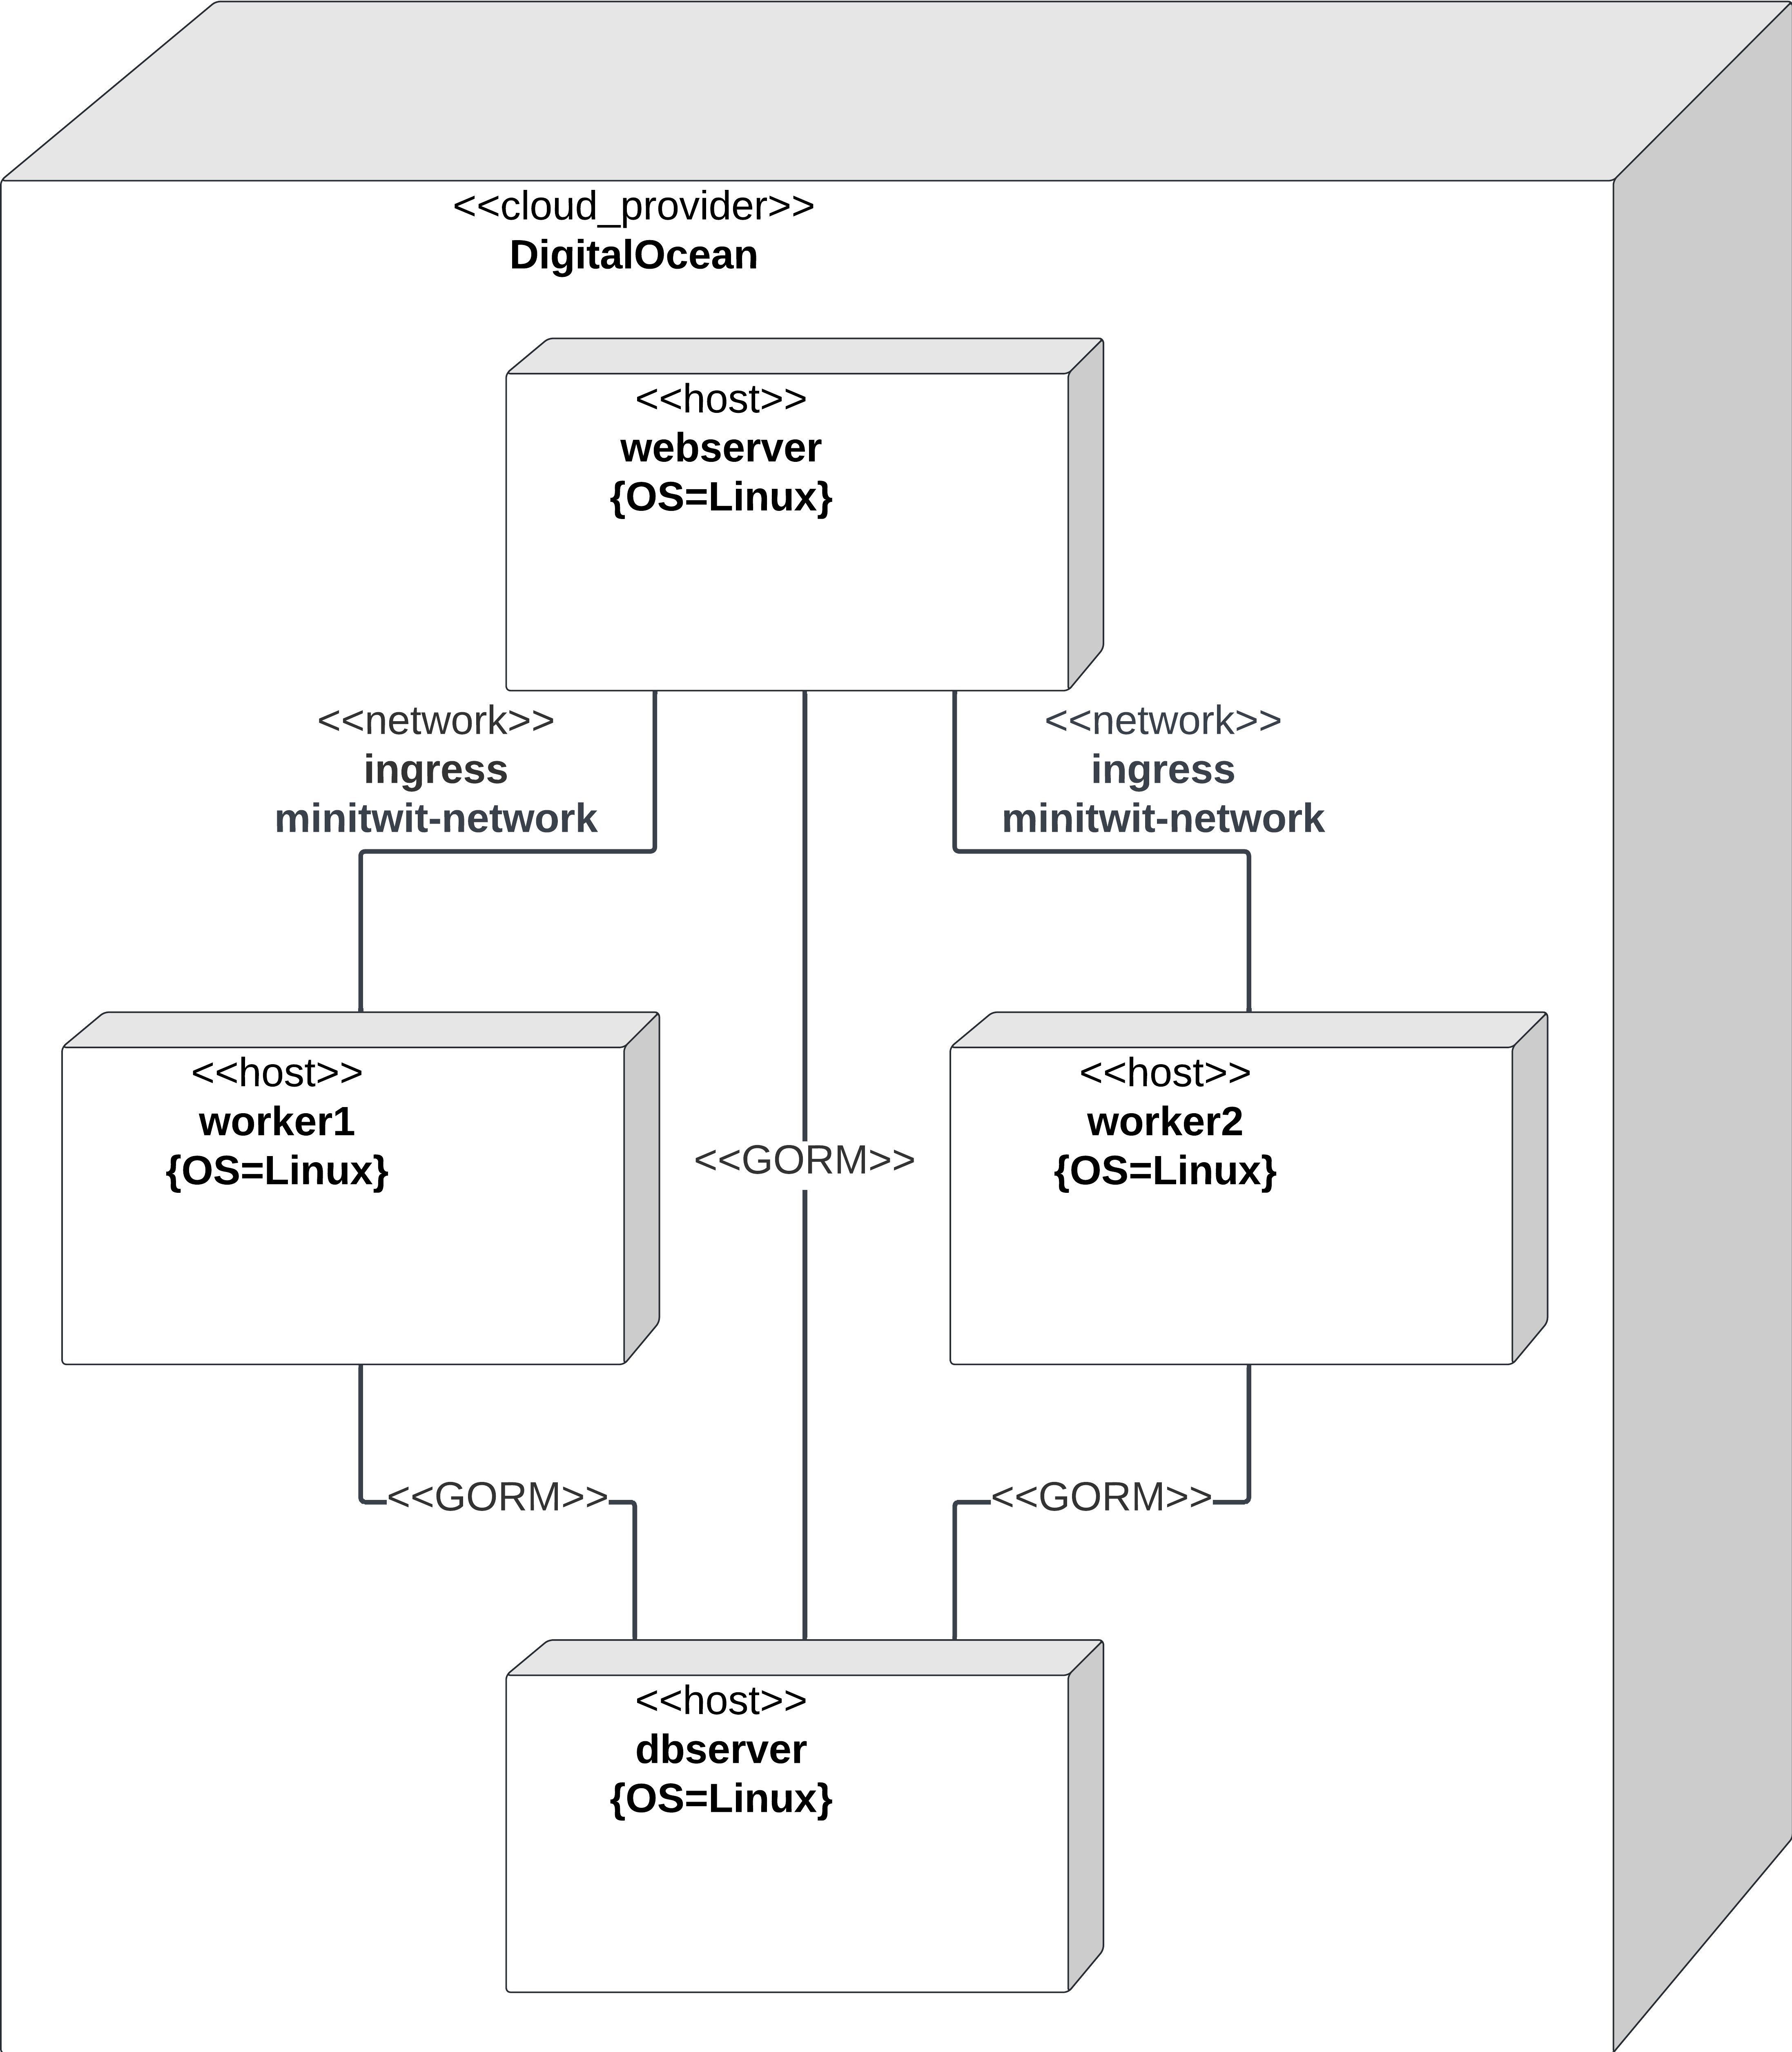
\includegraphics[width=0.6\linewidth]{images/uml-component-servers.png}
    \caption{Diagram displaying the different servers in the architecture with relations.}
    \label{fig:uml-servers}
\end{figure}

\subsection{Containers}
Zooming in on the \textit{webserver} reveals 2 different networks and 9 different containers running on this server.
Figure \ref{fig:uml-containers} displays the containers running on the server.

\begin{figure}[H]
    \centering
    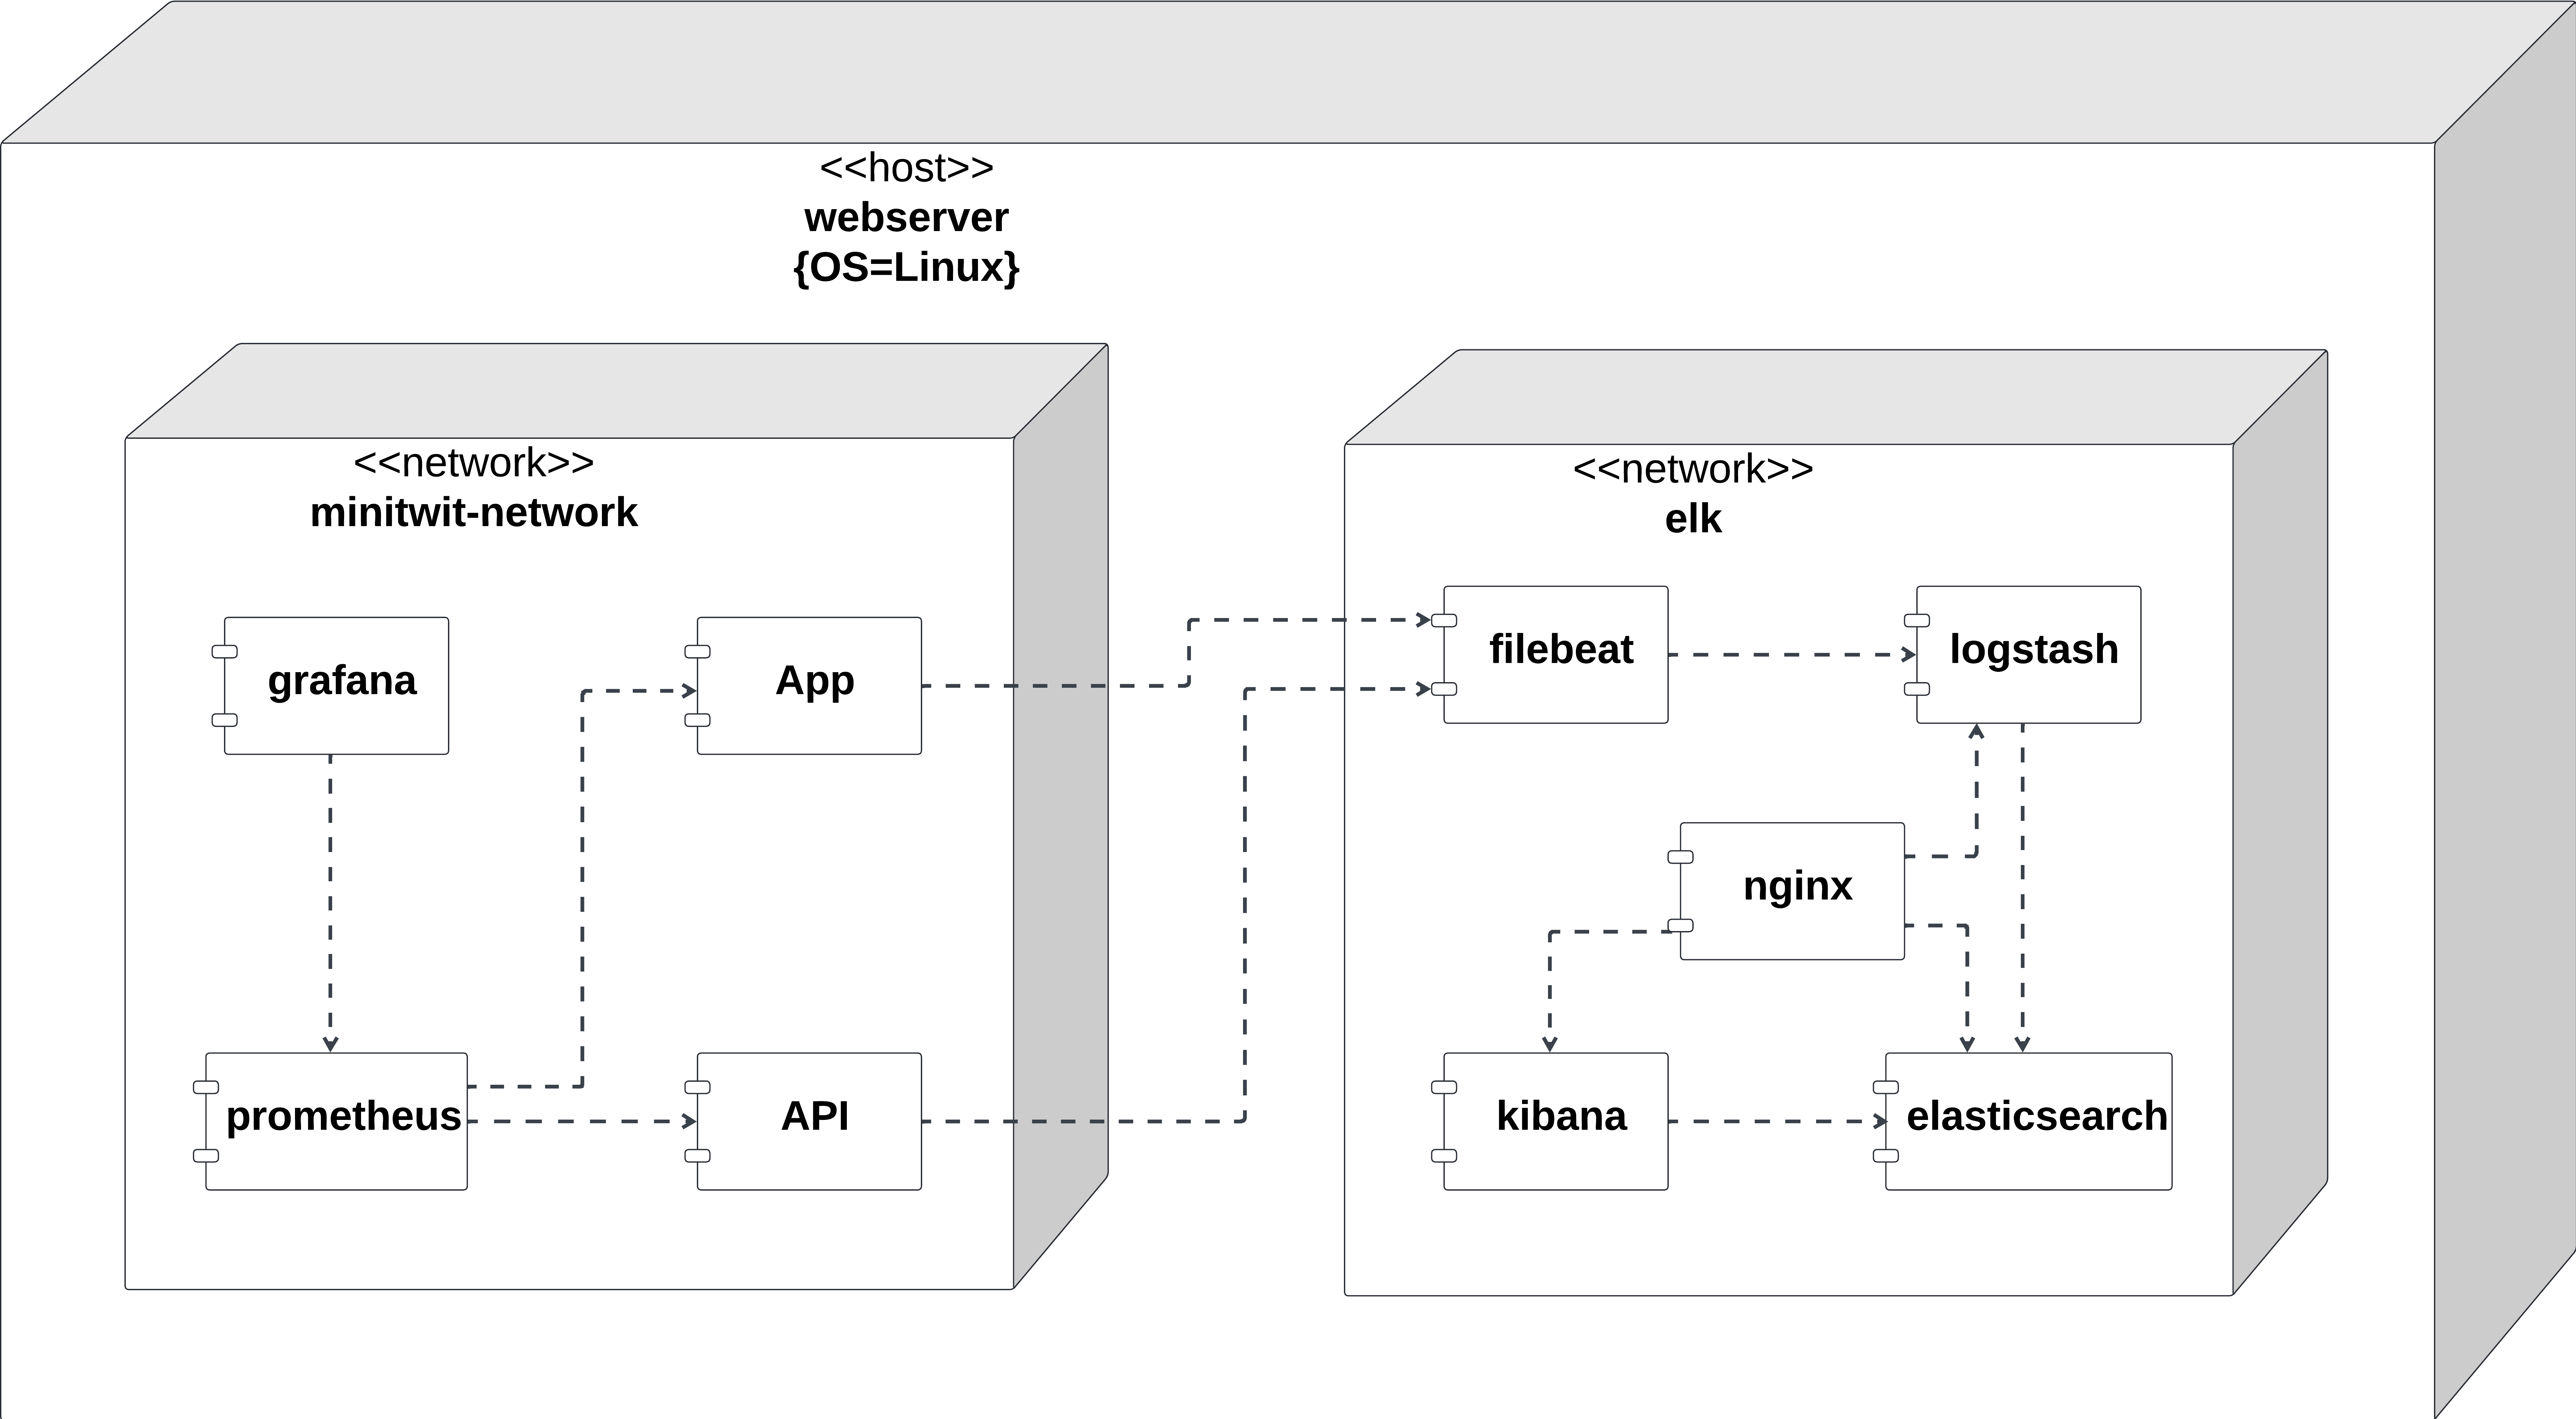
\includegraphics[width=0.8\linewidth]{images/uml-component-containers.png}
    \caption{Component diagram emphasizing the different containers in the architecture with relations}
    \label{fig:uml-containers}
\end{figure}

\subsection{App}
The following describes the structure of the \textit{App} container displayed in the services.
It includes several packages, all located in the src directory.
A package diagram that visualizes the app's structure is displayed in Figure \ref{fig:package-diagram-app}.
\textit{main.go} is the executed file, which sets up the templates in the \textit{Web} package, establishes database connection with the \textit{Database} package, and sets up controllers in the \textit{Controller} package to endpoints.
The \textit{Controller} package queries the database with the \textit{Database} package, adds popup notifications with the \textit{Flash} package, and creates ORM models with the\textit{Models} package.

\begin{figure}[H]
    \centering
    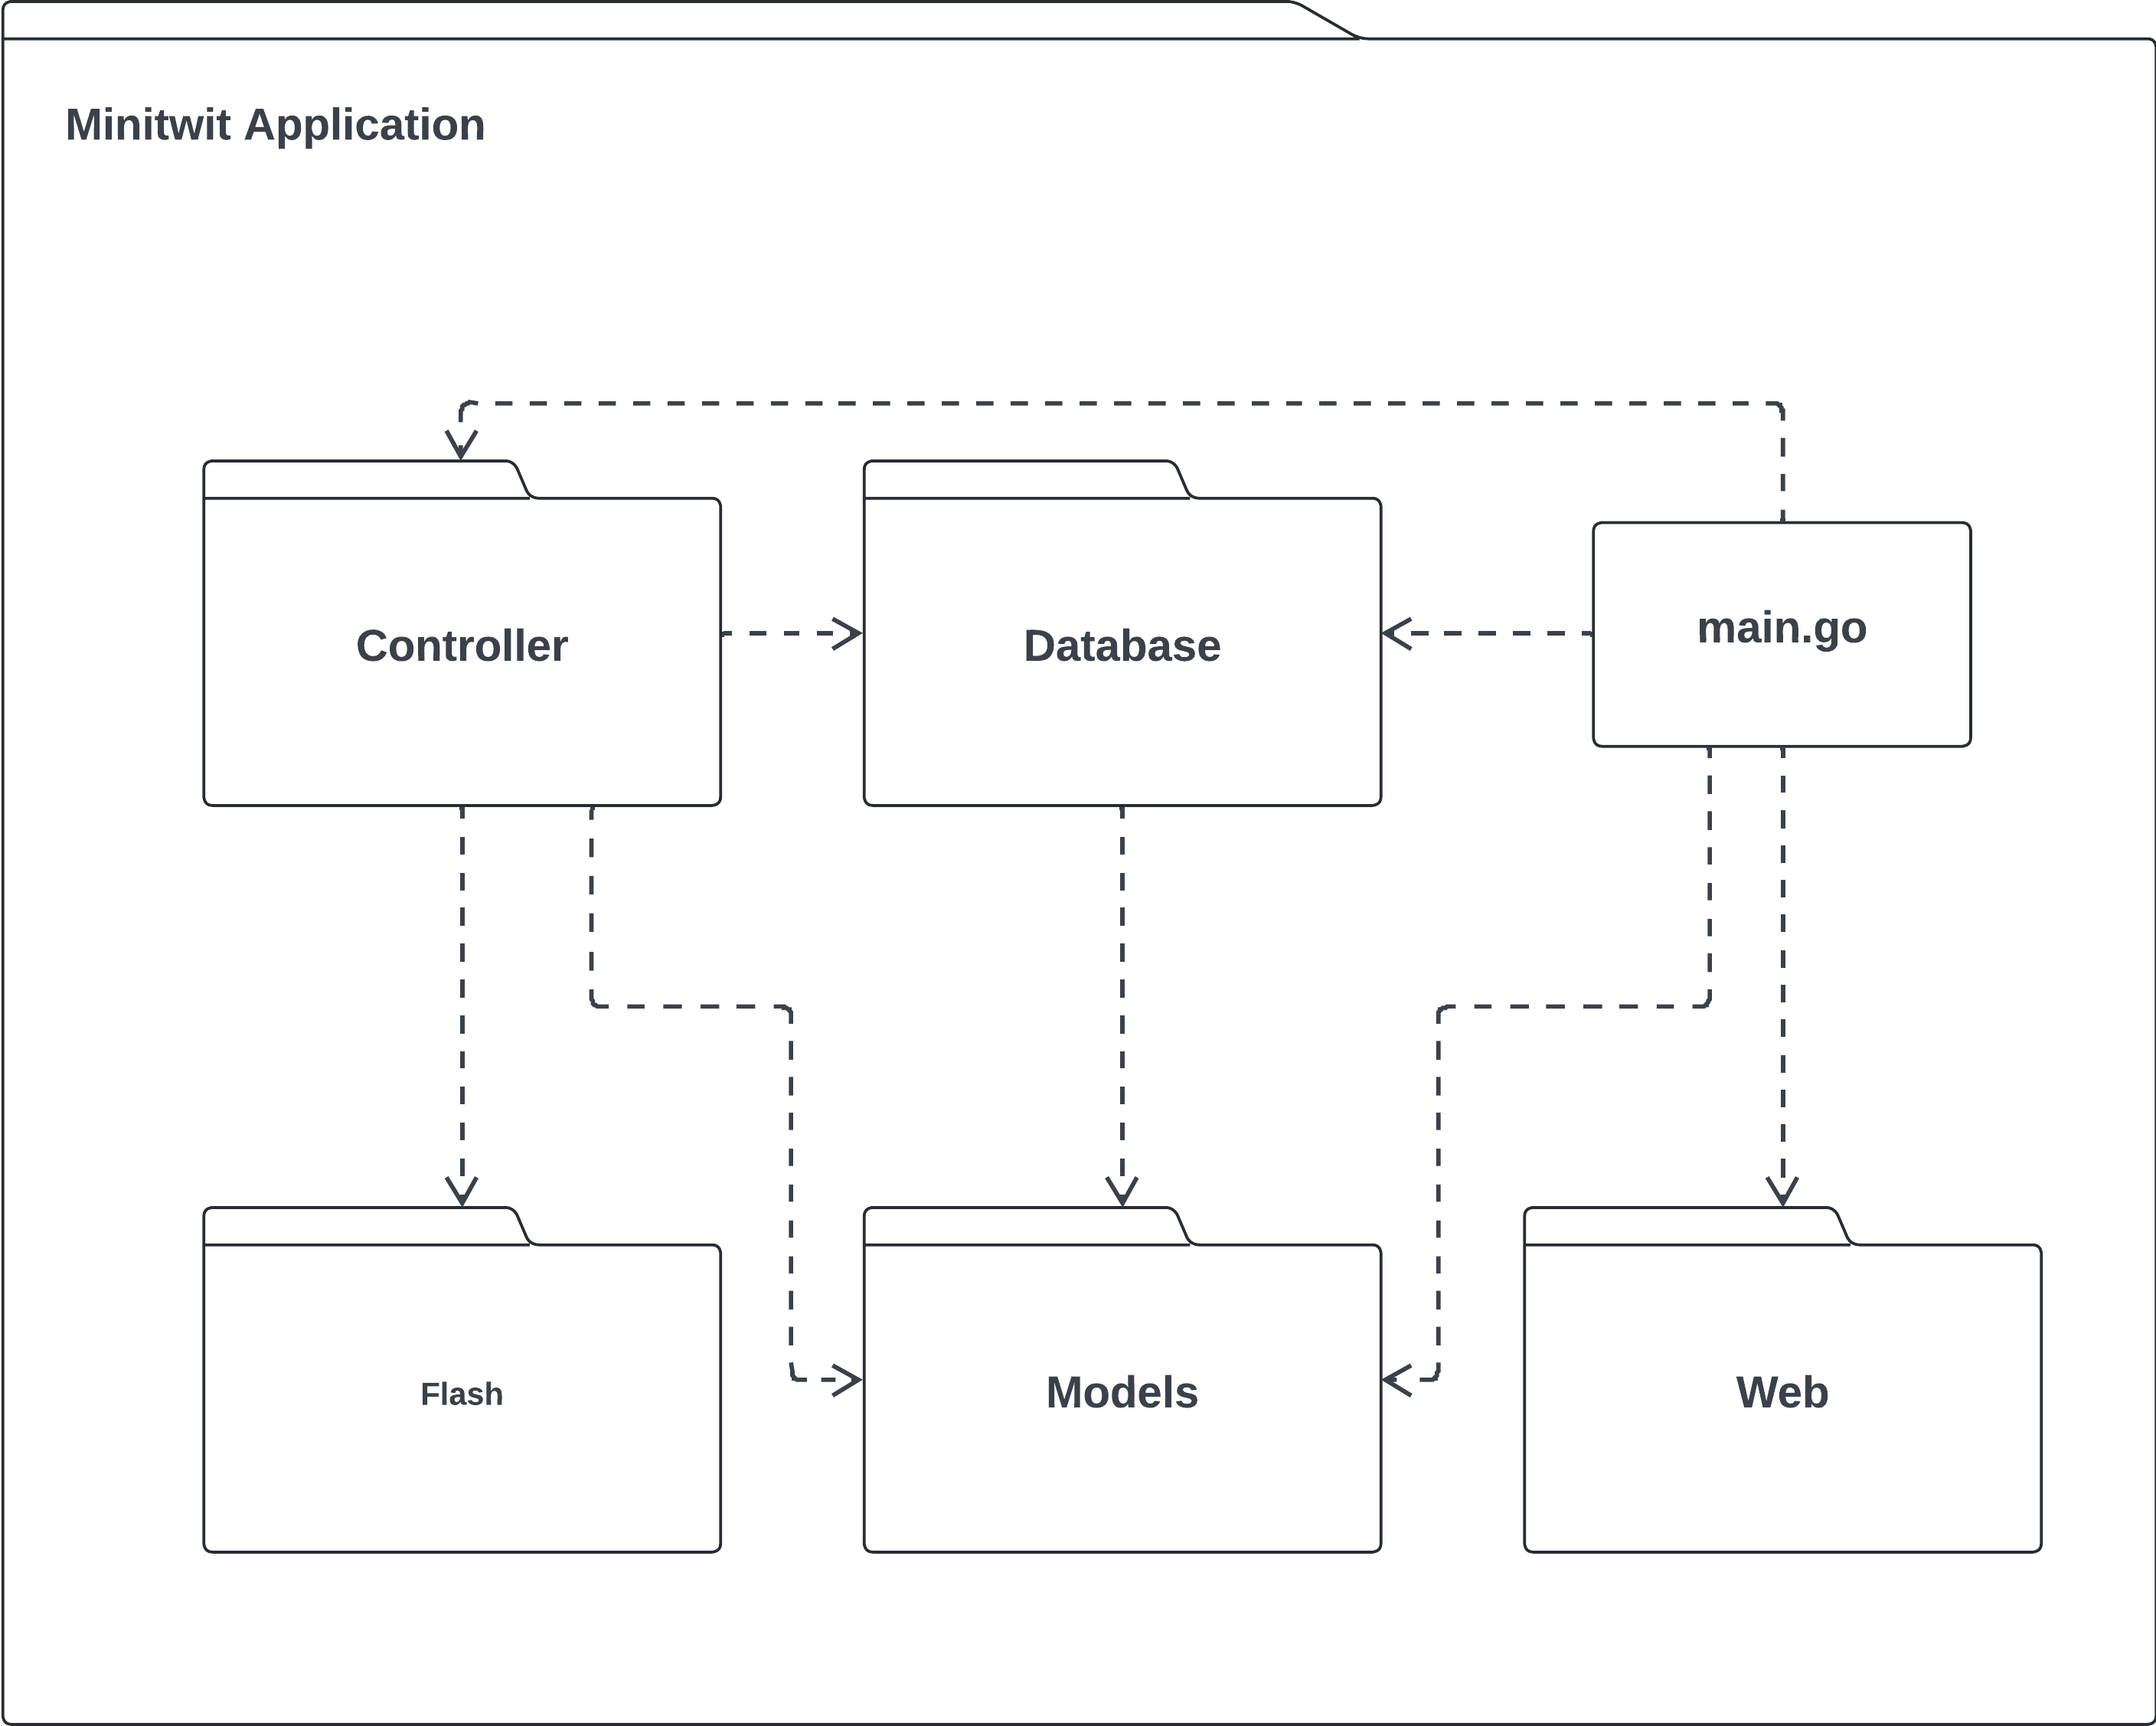
\includegraphics[width=0.6\linewidth]{images/uml-package-app.png}
    \caption{Package diagram of the main application running on the App service}
    \label{fig:package-diagram-app}
\end{figure}

\section{Dependencies of the Minitwit system}

This section will detail all the technologies, tools, and external services our system depends on, categorized for clarity.

\subsection{Monitoring}\label{sec:monitoring-architecture}
The system is monitored with Grafana and Prometheus, with the stack depicted in Figure \ref{fig:monitoring-stack}.
Prometheus is the data collector, pulling metrics from the app and API.
Grafana queries these metrics and visualizes relevant stats for maintenance.
Furthermore, Grafana also connects to the database to retrieve information about the tables in the database.

\begin{figure}[H]
    \centering
    \hbox{\hspace{-5em}
    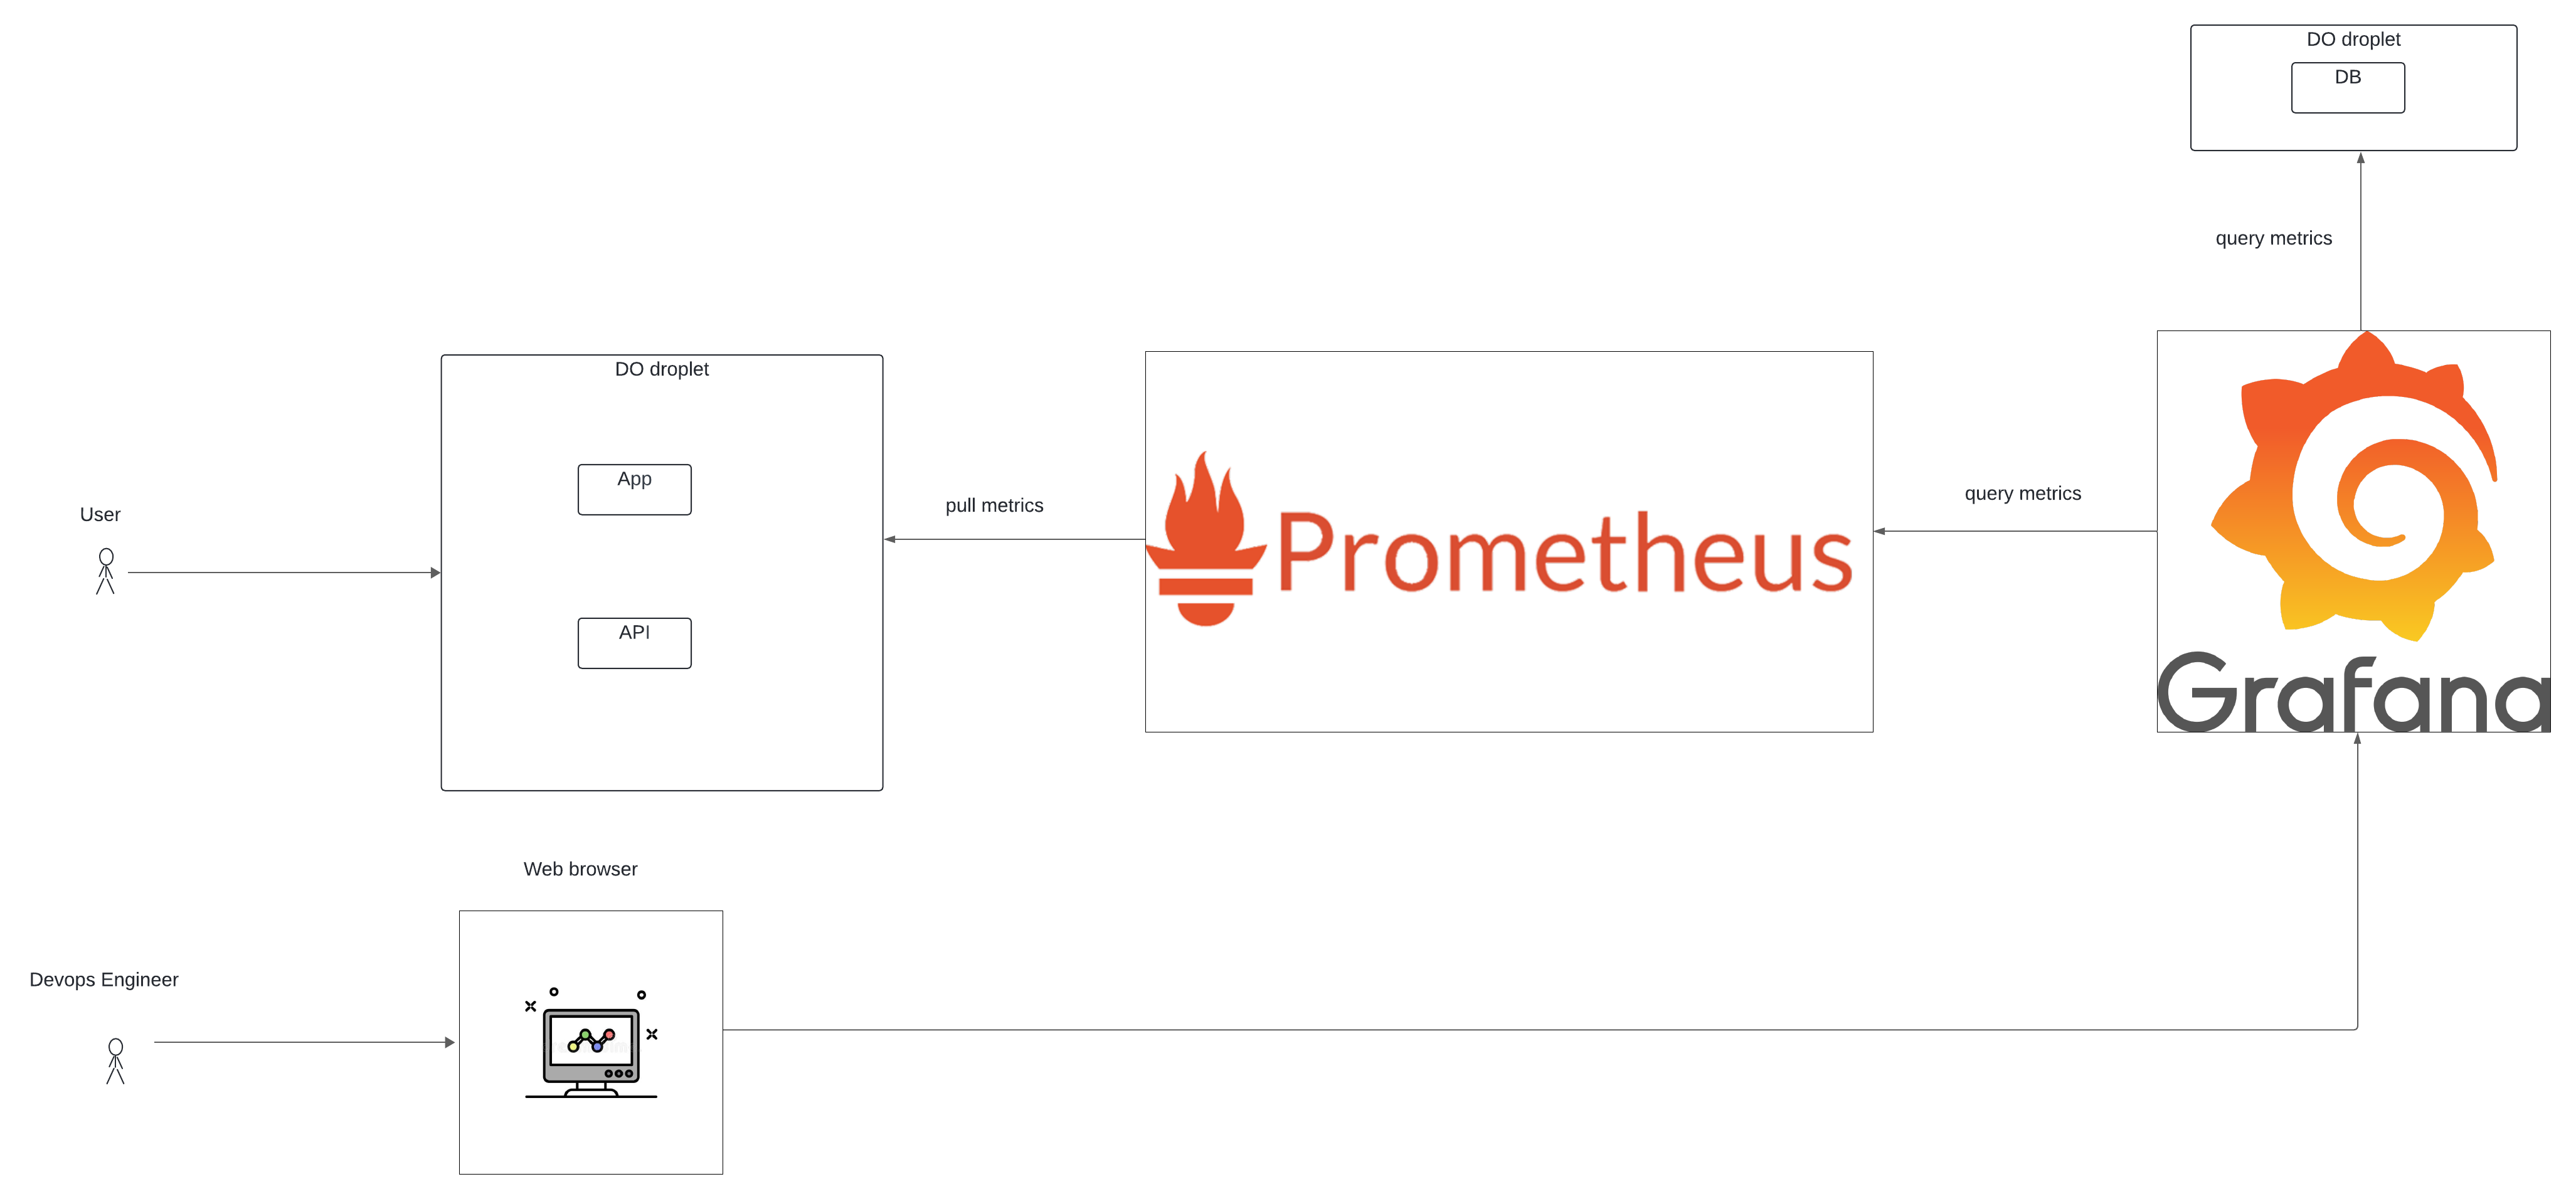
\includegraphics[scale = 0.3]{images/grafana.png}}
    \caption{Monitoring stack}
    \label{fig:monitoring-stack}
\end{figure}

\subsection{Logging}\label{sec:logging-architecture}

In Figure \ref{fig:elk-stack}, you can see how our ELKB stack is structured to ship logs to Elasticsearch and further analyze them.
\begin{figure}[H]
    \centering
    \hbox{\hspace{-6em}
    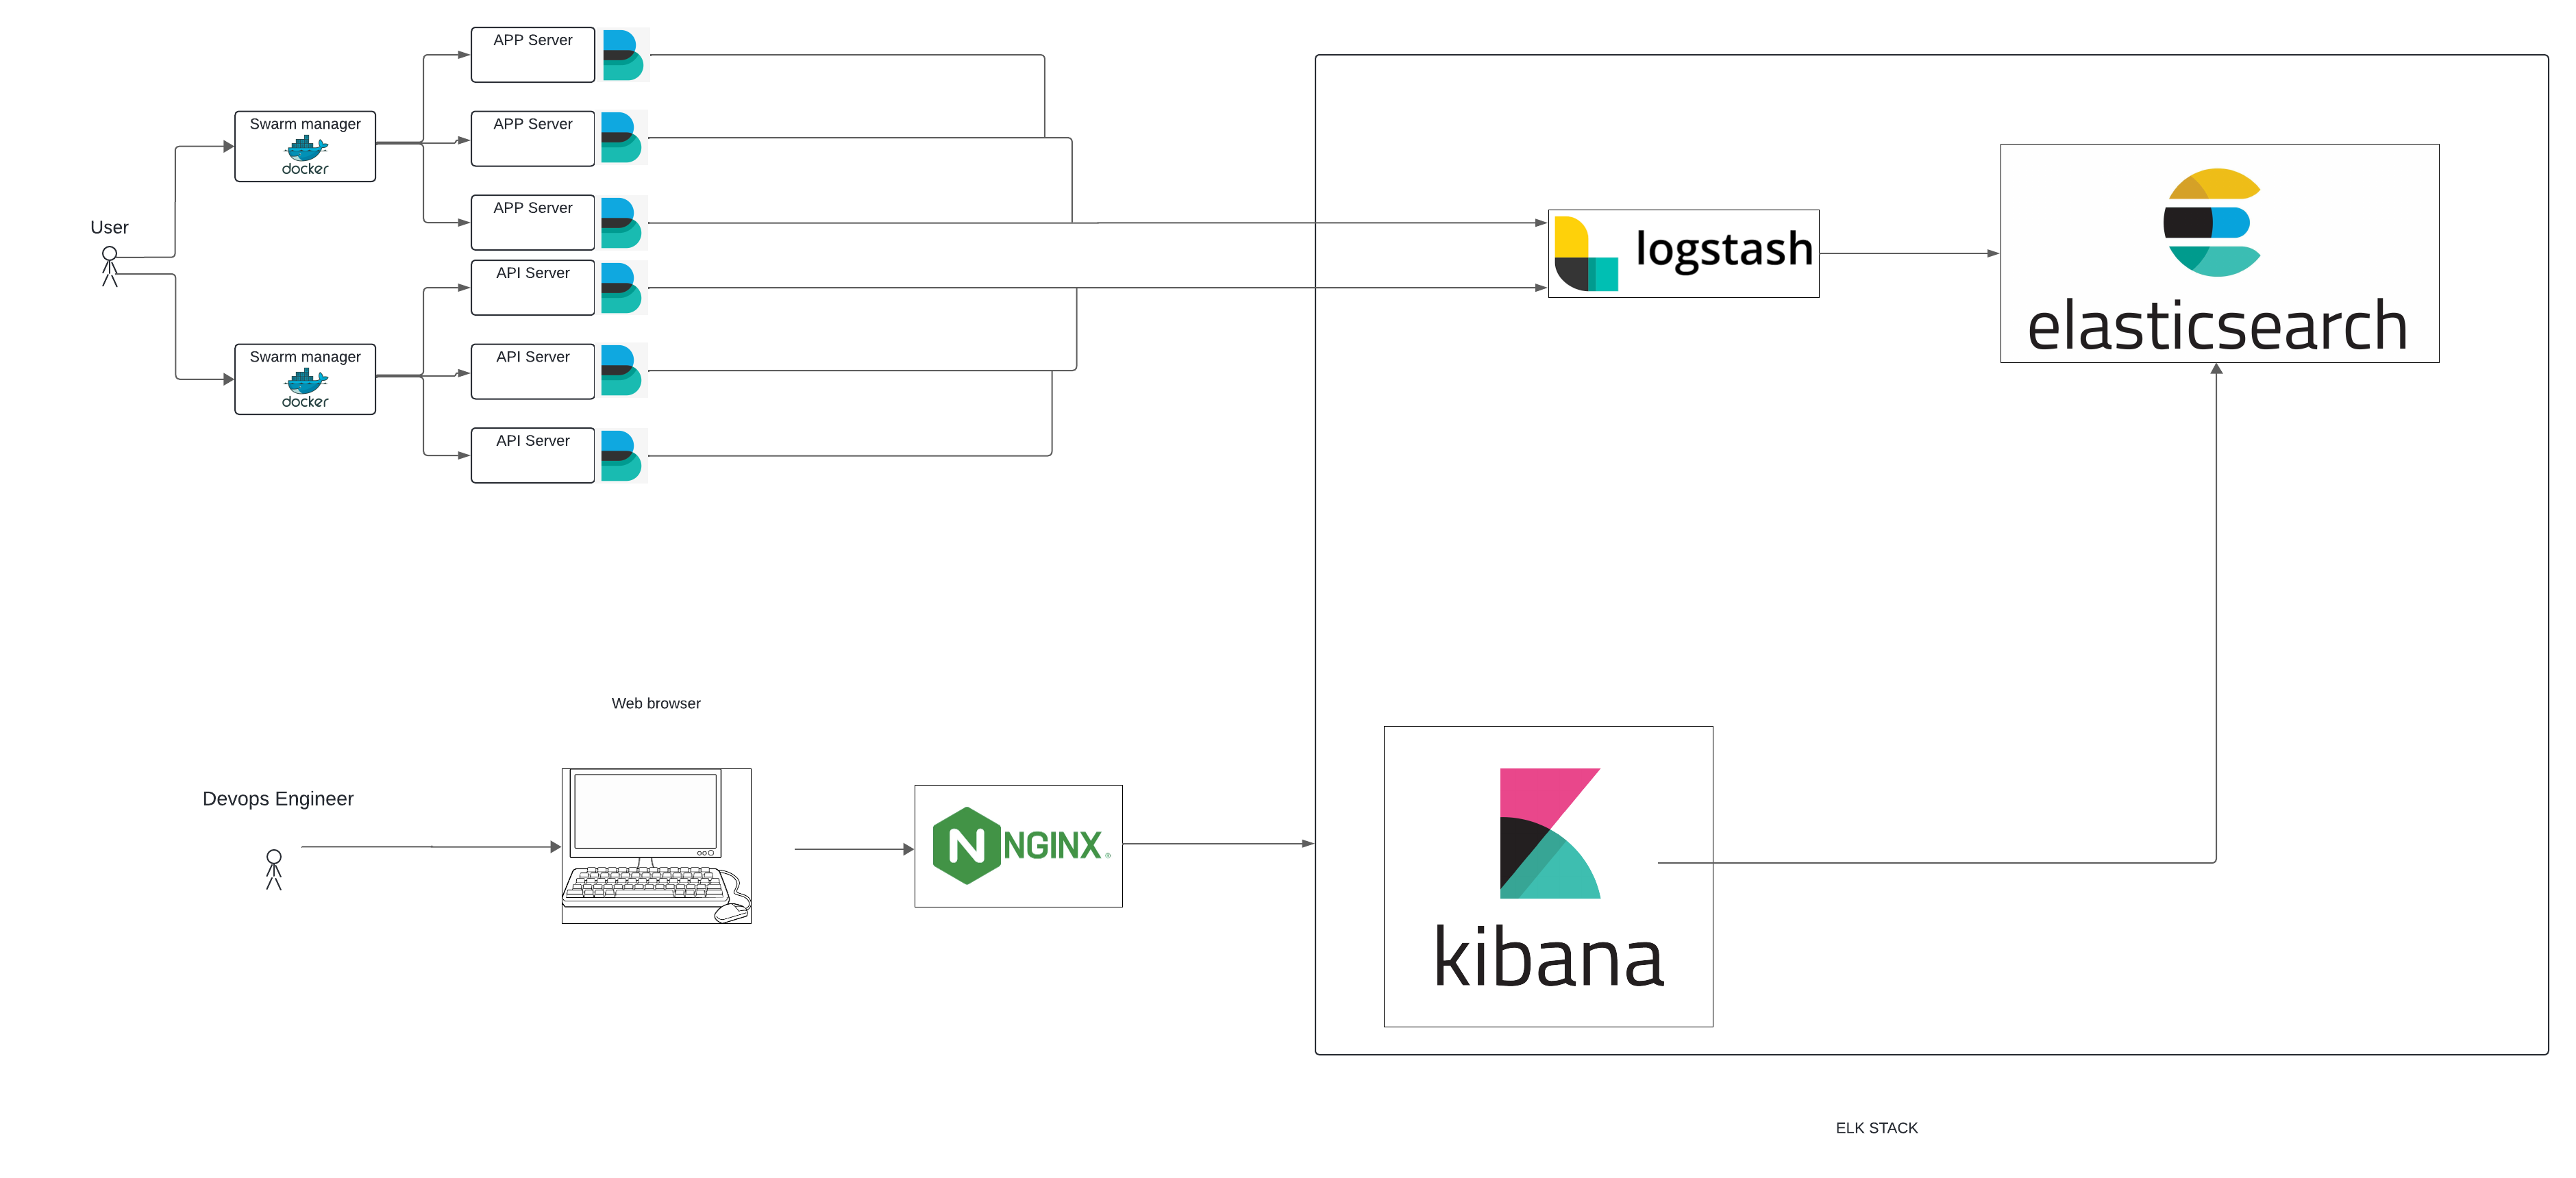
\includegraphics[scale = 0.37]{images/elk.png}}
    \caption{ELK stack}
    \label{fig:elk-stack}
\end{figure}

A label tag added to our \textit{App} and \textit{API} services enables Filebeat to auto-discover logs from those containers, which have that option enabled. Filebeat will collect logs only containing a timestamp, which are those generated by the logger of our code, and ship them to Logstash where they will be further processed to be outputted to Elasticsearch.
Finally, the developer can analyze and visualize these logs through Kibana in the browser, where the stack will be reverse proxied by Nginx for authentication reasons. \bigskip

\subsection{Development Dependencies}
We used Git and GitHub as the development version control and collaboration tools, and GitHub Organizations to manage the project with the “Projects” feature. 
GitHub Actions and Sonarcloud were used with workflows on pull requests to the \textit{main} branch, automating the CI/CD process and analysis of code quality.\bigskip

We used Terraform as the IaC, allowing for a simple IaC setup, with a \textit{tfvars} file to include environment variables efficiently.
All processes in the system are containerized with Docker to work without any dependency issues, using mainly docker-compose to orchestrate the services.\bigskip


\subsection{Runtime Dependencies}
The application is hosted in a Linux server inside a DigitalOcean droplet, where it is containerized with Docker.
The application and API connect to a Postgres database with GORM, a Golang ORM framework.
The database can easily be replaced due to a volume connected to the container storing the data.
The application and API are built with Golang and utilize the \textit{Gin} dependency, an HTTP web application package.

\section{Important interactions of subsystems}

\subsubsection{Information Flow of the Web Application}
The diagram in Figure \ref{fig:seq-diagram-infoflow} showcases the system traversal of submitting a message.
When a user submits a message, the system makes a POST request to our web server, which routes the request to the controller, where it performs all the logic.
Afterwards, the proper status code is returned.

\begin{figure}[H]
    \centering
    \fbox{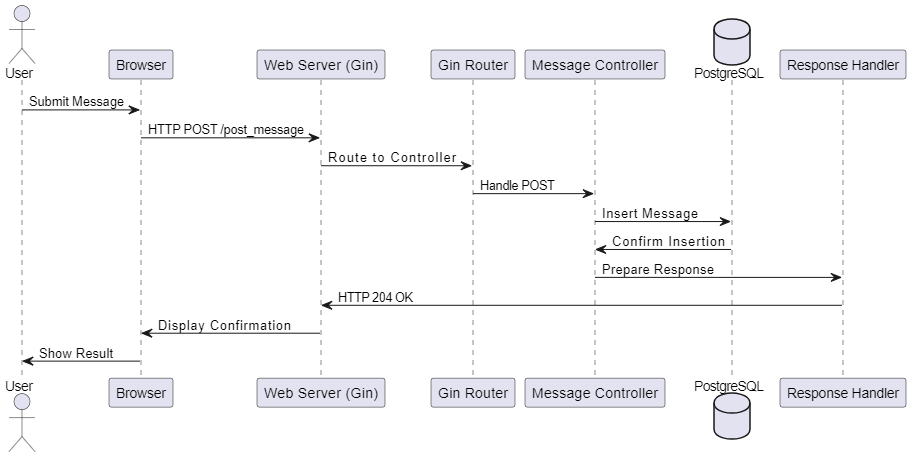
\includegraphics[width=\textwidth]{images/uml-seq-infoflow.png}}
    \caption{Sequence diagram of information flow of submitting a message in the application.}
    \label{fig:seq-diagram-infoflow}
\end{figure}

\subsubsection{Flow of API Endpoints}
Figure \ref{fig:seq-diagram-register} displays how the simulator traverses the register endpoint, including exception handling of unfilled register form and username already registered.

\begin{figure}[H]
    \centering
    \fbox{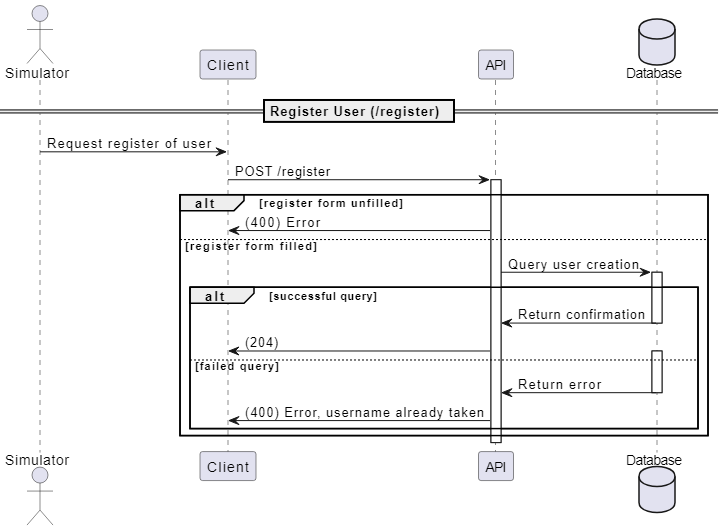
\includegraphics[width=0.6\textwidth]{images/uml-seq-register.png}}
    \caption{Sequence diagram displaying the traversal of the \texttt{POST /register} endpoint of the API.}
    \label{fig:seq-diagram-register}
\end{figure}

\begin{figure}[H]
    \centering
    \fbox{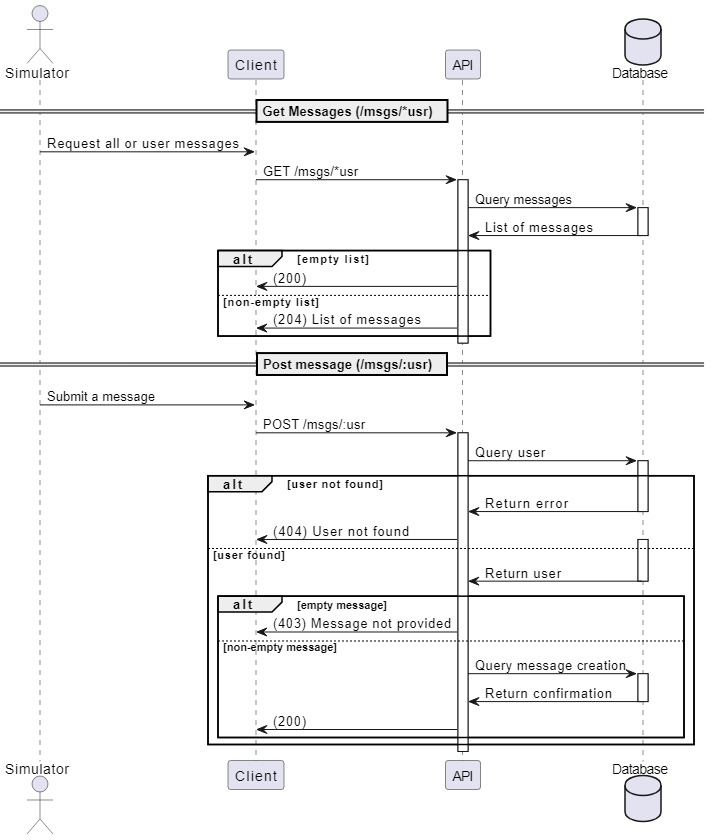
\includegraphics[width=0.7\textwidth]{images/uml-seq-message.png}}
    \caption{Sequence diagram displaying the traversal of the \texttt{/msgs} endpoints, including \texttt{GET /msgs/*usr} and \texttt{POST /msgs/:usr}, of the API.}
    \label{fig:seq-diagram-message}
\end{figure}

\newpage

Figure \ref{fig:seq-diagram-message} displays the traversal of the \texttt{/msgs} endpoints, including error handling with unregistered users and empty messages.
An important distinction is between the \texttt{usr}, where \texttt{*} indicates an optional user (fetching all messages if not provided), and \texttt{:} indicates a required user.

Figure \ref{fig:seq-diagram-follow} depicts the traversal of the \texttt{/fllws} endpoints, error handling at unregistered users, insufficient JSON format for the ORM, and if the query fails.
Unsuccessful follow will return 400, and unsuccessful unfollow will return 403.

\begin{figure}[H]
    \centering
    \fbox{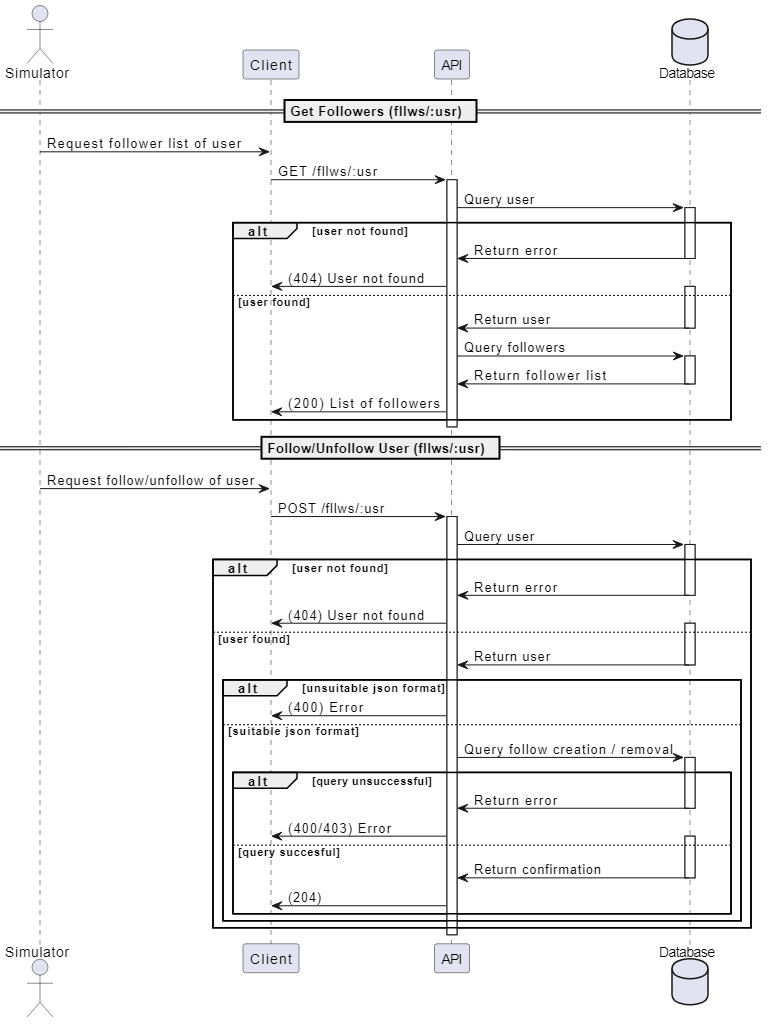
\includegraphics[width=0.8\textwidth]{images/uml-seq-follow.png}}
    \caption{Sequence diagram displaying the traversal of the \texttt{/fllws} endpoints, including \texttt{GET fllws/:usr} and \texttt{GET /fllws/:usr}, of the API.}
    \label{fig:seq-diagram-follow}
\end{figure}

\newpage

\section{Current state of the system}

All artifacts of the system are linked in Appendix \ref{app}.

\subsection{Static Analysis}

We use SonarCloud for static analysis, performing scans automatically on pull requests. It identifies code smells, security and maintainability issues etc. Current issues are most low to moderate severity, mostly concerning maintainability, and should only require minor updates. Dependency health is good. The only security issues identified concern the use of recursive copying in a Dockerfile.

\subsection{Test coverage}

In the build stage of our CI/CD pipeline we test all the API endpoints, except for the “root”, “version” and “metrics” endpoints with both positive and negative test cases, ensuring that the API should work according to the users expectations. Unit tests have not been implemented.

\subsection{Performance}

From our Grafana Dashboard, we can see that requests to our API currently take $\sim 9\,\text{ms}
$ for the $99\text{th}$ percentile of requests. Unfortunately, the app webpage takes $\sim 6$ seconds to process requests, an issue that warrants further inspection.

\subsection{Observability and Monitoring}
In our logs, we have not detected any unusual activity. Monitoring and logging is further discussed in Sections~\ref{sec:Monitoring} and~\ref{sec:Logging}.

\chapter{Process' perspective}

\section{CI/CD Chain}
We implemented a GitHub Actions workflow to automate the process of testing, building and deploying the most recent version of Minitwit, set to execute on each pull request to the \textit{main} branch of our GitHub repository.
The workflow is separated into three jobs: \textit{BuildAndTest}, \textit{Deploy}, and \textit{Release}, which are codependent and executed sequentially,  \bigskip

A comprehensive deployment diagram describing the build and deployment part of the CI/CD applied with GitHub Actions is displayed in Figure \ref{fig:deployment-cicd-minimal}.\bigskip

\begin{figure}
    \centering
    \includegraphics[width=\linewidth]{images/uml-deployment-githubactions.png}
    \caption{Deployment Diagram of deploying with a pull request or manually on GitHub Actions.}
    \label{fig:deployment-cicd-minimal}
\end{figure}

\newpage

\subsection{Jobs}
\subsubsection{BuildAndTest}
All relevant images are built and pushed to DockerHub and then tested to ensure the system works. The key steps are:

\begin{enumerate}
    \item \textbf{Checkout} 
    \begin{itemize}
        \item Uses \texttt{actions/checkout@v2} to fetch the codebase from the repository.
    \end{itemize}
    
    \item \textbf{Environment Setup} 
    \begin{itemize}
        \item Creates a \texttt{.env} file with database configurations sourced from GitHub secrets.
    \end{itemize}
    
    \item \textbf{Docker Operations}
    \begin{itemize}
        \item Logs into Docker Hub using credentials from GitHub secrets to push built images, including:
        \begin{itemize}
            \item The application image
            \item API image
            \item A test database image
        \end{itemize}
    \end{itemize}
    
    \item \textbf{Python Setup and Dependency Installation}
    \begin{itemize}
        \item Configures the Python environment and installs necessary dependencies.
    \end{itemize}
    
    \item \textbf{Testing}
    \begin{itemize}
        \item Executes integration tests by setting up the application and its dependencies in Docker containers.
        \item Conducts API tests and application-specific tests.
    \end{itemize}
\end{enumerate}

\subsubsection{Deploy}
The \textbf{Deploy} job is activated on successfully completing the \textbf{BuildAndTest} job.
It deploys the application to the remote server where it is hosted.
The steps are:

\begin{enumerate}
    \item \textbf{Checkout} 
    \begin{itemize}
        \item Fetches the codebase from the repository, uses \texttt{actions/checkout@v2} similar to the first job.
    \end{itemize}
    \item \textbf{SSH Configuration} 
    \begin{itemize}
        \item Prepares SSH keys for connection to the deployment server.
    \end{itemize}
    
    \item \textbf{Deployment Execution}
    \begin{itemize}
        \item Updates environmental configurations and transfers necessary files to the server using SCP.
        \item Pulls the latest Docker images from the Docker Compose file.
        \item Deploys the images using Docker Stack, updating the running application on all servers in the Docker swarm.
    \end{itemize}
\end{enumerate}

 \subsubsection{Release}
 Manages software versioning and public release.

 \begin{enumerate}
    \item \textbf{Version Calculation:}
    \begin{itemize}
        \item Executes a script to determine the version number for automated version tracking.
    \end{itemize}
    
    \item \textbf{GitHub Release Creation:}
    \begin{itemize}
        \item Uses \texttt{actions/create-release@v1} to create a formal release on GitHub.
        \item Tags the release with the new version number and provides release notes.
    \end{itemize}
\end{enumerate}

\section{Monitoring}
\label{sec:Monitoring}
We use Prometheus to collect and integrate metrics with Grafana to visualize key metrics live. Additionally, Grafana queries the database to visualize the data stored.
We have two dashboards, one monitoring the API and the other the database.
Both dashboards are passive monitoring, sniffing the simulated users' HTTP requests\cite{furnari2014}.
They are also both considered proactive monitoring by measuring application performance\cite{turnbull2015}, and both are considered whitebox\cite{turnbull2016} since they are applied inside the codebase.
DigitalOcean also includes infrastructure monitoring with real-time bandwidth, CPU usage, and disk I/O graphs, as depicted in Figure \ref{fig:do-monitoring}.

\begin{figure}[H]
    \centering
    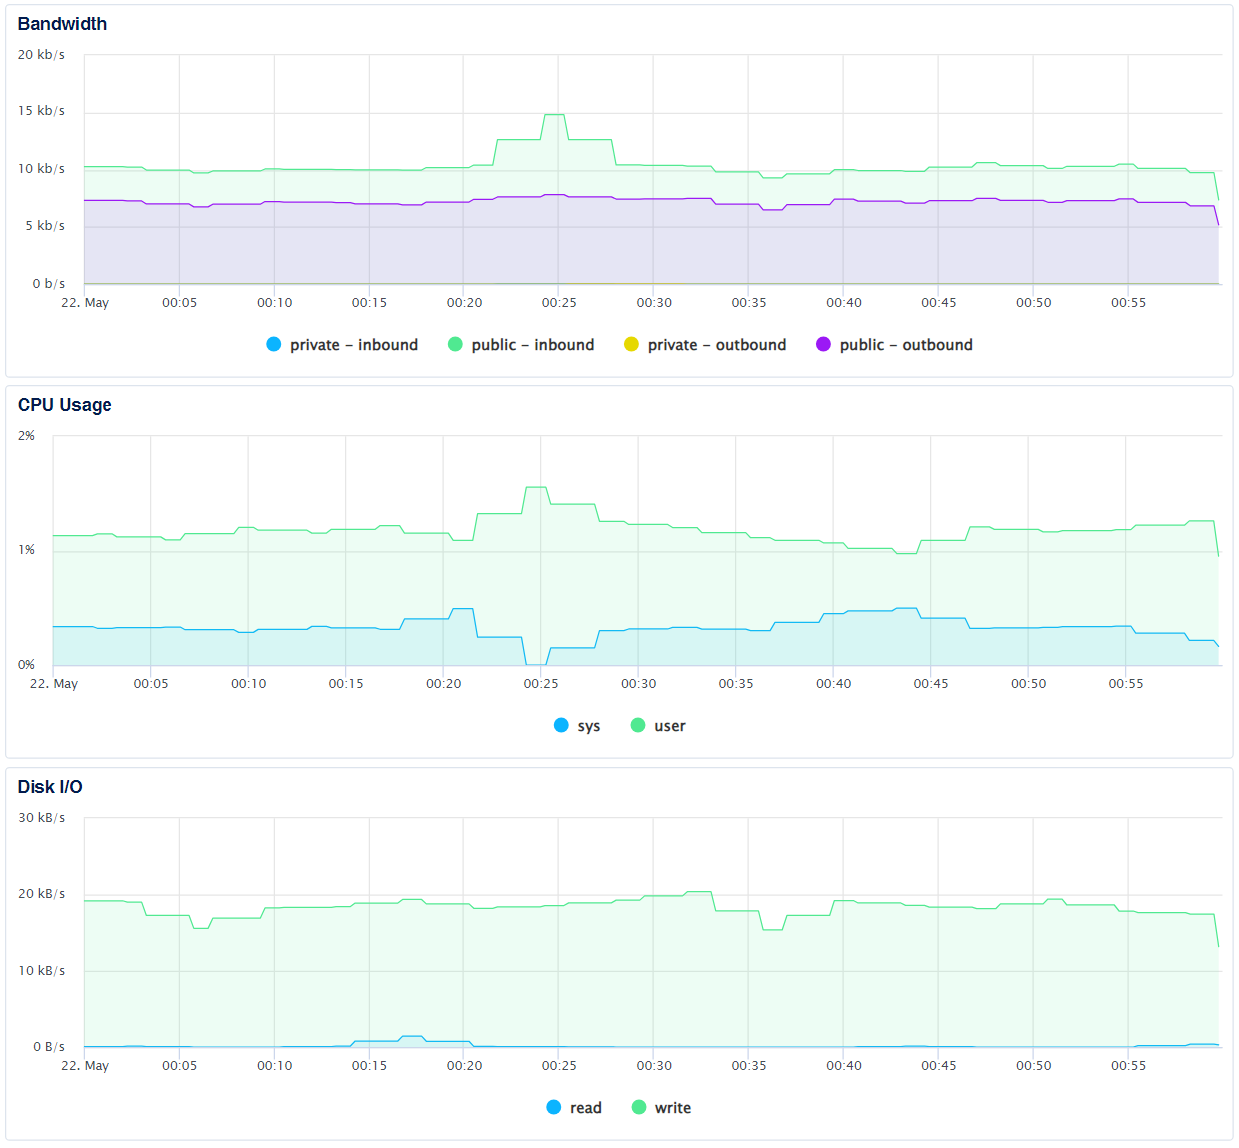
\includegraphics[width=0.7\linewidth]{images/do-monitoring.png}
    \caption{DigitalOcean Monitoring}
    \label{fig:do-monitoring}
\end{figure}

\subsection{API dashboard}
The API dashboard mainly focuses on determining which HTTP requests are incoming from the API, prioritized due to the simulator using the API.
The dashboard collects data from Prometheus.
The monitoring uses an application monitoring tactic, monitoring how well the API responds to requests and which requests occur\cite{julian2018}.
The metrics from Prometheus are pulled from the code, which pushes all metrics into an API endpoint, so it is somewhat of a hybrid monitoring.
Figure \ref{fig:api-dashboard} displays the API monitoring dashboard.

\begin{figure}[H]
    \centering
    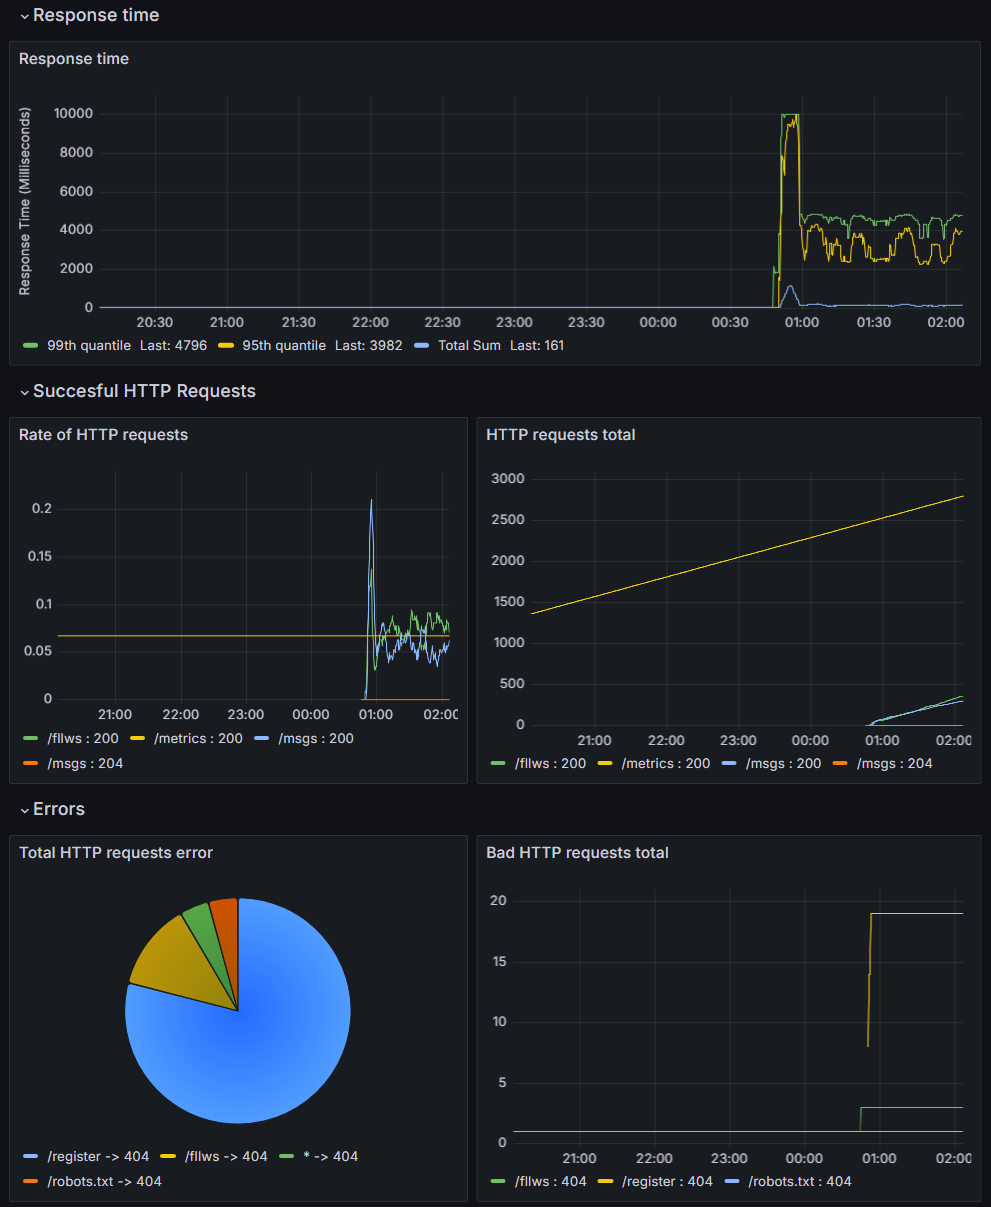
\includegraphics[width=0.7\linewidth]{images/api-dashboard.png}
    \caption{API Dashboard in Grafana}
    \label{fig:api-dashboard}
\end{figure}

\subsection{Database dashboard}
The database dashboard visualizes stats about what is currently obtained in the database by querying the database directly from Grafana.
The database monitoring acts like a 'monitoring the business' tactic by visualizing information about the number of users and messages there are and revealing distributions that may be useful for business~\cite{julian2018}.
The database statistics are considered pull-based since the database is queried to and, therefore, pulled from.
Figure \ref{fig:db-dashboard} displays the database monitoring dashboard.

\begin{figure}[H]
    \centering
    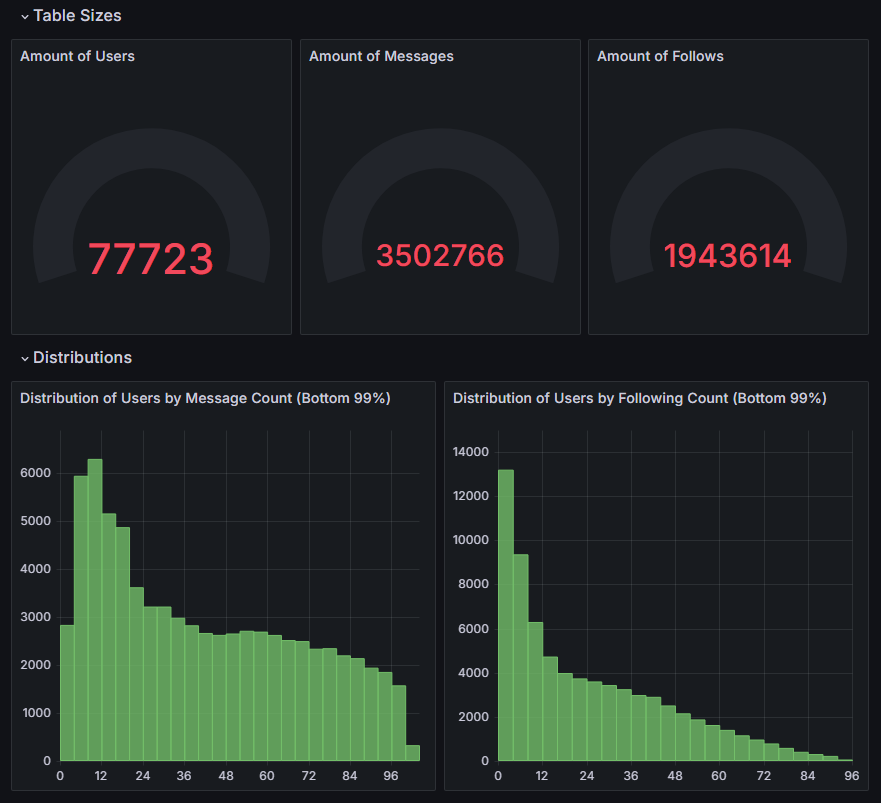
\includegraphics[width=0.8\linewidth]{images/database-dashboard.png}
    \caption{Database Dashboard in Grafana}
    \label{fig:db-dashboard}
\end{figure}

\section{Logging}
\label{sec:Logging}
The main events of the application and API are logged using 4 levels: info, debug, error, and fatal. We used the “info” level to communicate the events in a general level of how things are happening; “debug” for debugging purposes, how parameters are being changed and passed; “error” when the program encounters some non-fatal errors for example, in our Go app when the “err” parameter is not nil we notify it with the error level; finally “fatal” is used for errors that halt or crash the application. \bigskip

All logs are collected in a single index pattern from all sources from the “app” and “application.
We can distinguish the sources in Kibana because you can see from which folder and which file the log is generated, depicted in Figure \ref{fig:kabana-logs}.
\begin{figure}[H]
    \centering
    \hbox{\hspace{-5em}
    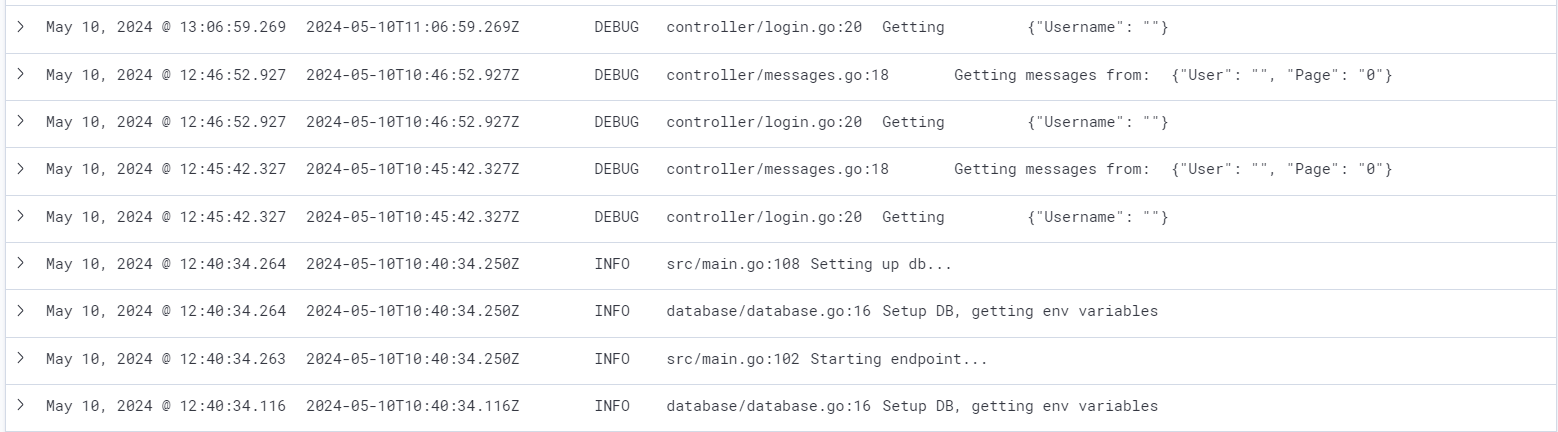
\includegraphics[scale = 0.6]{images/kibana.png}}
    \caption{Logs from Kibana}
    \label{fig:kabana-logs}
\end{figure}

\section{Security assessment}
The application components are as described in chapter~\ref{chap:System's Perspective} section 
~\ref{sec:Design and architecture of the Minitwit system}. 

The user data that we store in our database are username, password, and email.
The username and email are public information and are therefore not sensitive data.
Depending on the user, and if they are reusing their password on multiple applications, the password is not sensitive data.

\begin{figure}[H]
    \centering
    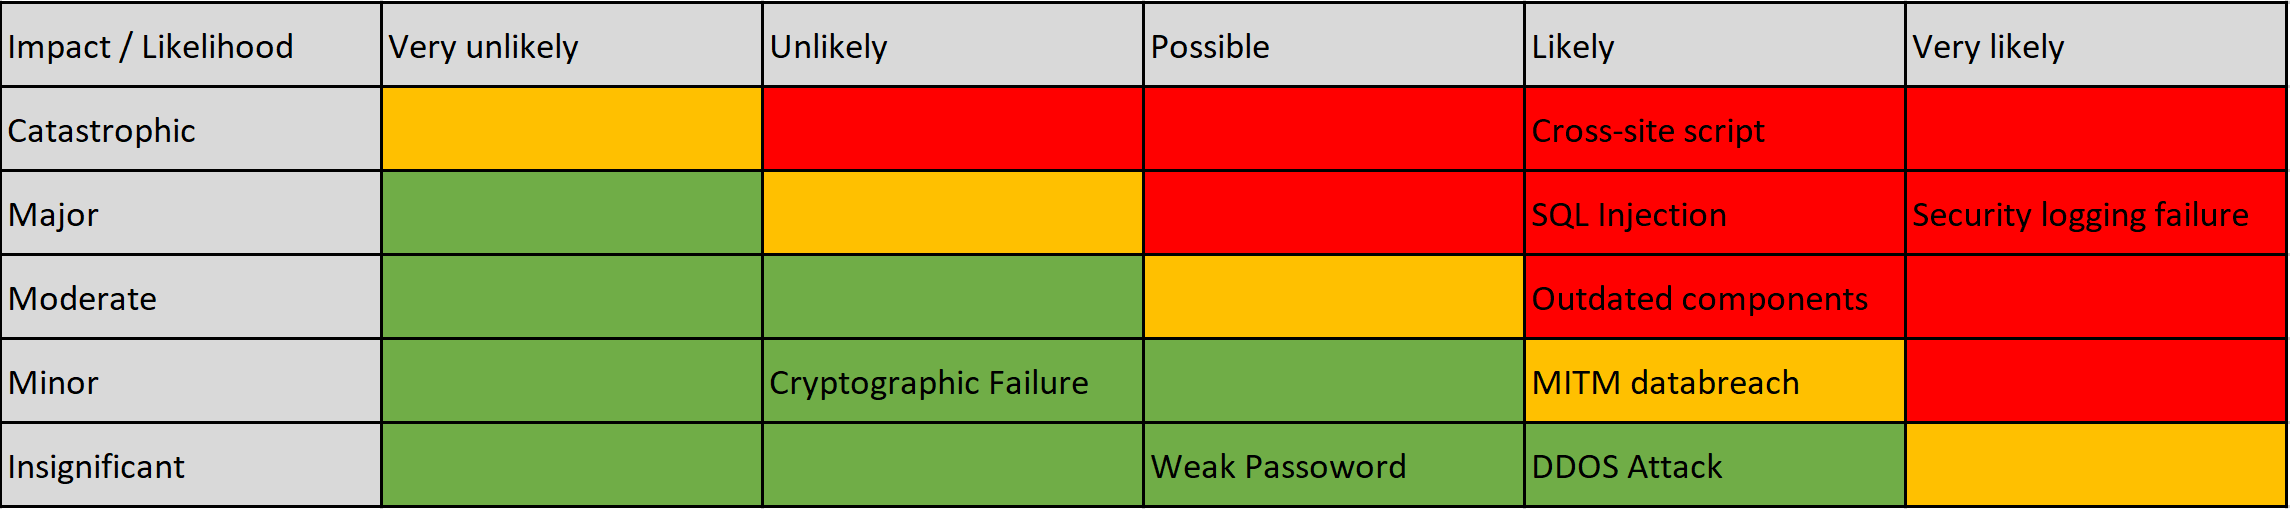
\includegraphics[width=1.0\textwidth]{images/SecRiskAssMatrix.PNG}
    \caption{Security risk assessment matrix\cite{owasp2024}\cite{comparitech2024}}
    \label{fig:security matrix}
\end{figure}


\section{Scaling strategy}
The system induced both horizontal and vertical scaling.
Horizontal scaling is implemented with Docker Swarm, with two additional worker replicas to assist and backup the single web server in its tasks from the app and API, which can easily be scaled by increasing workers.
The web server is the manager who delegates tasks to the workers and can handle tasks itself if delegation is unnecessary.\\
\\
Vertical scaling was implemented since Elasticsearch was very performance-heavy; as a quick solution, the web server was scaled vertically with more memory from 1 to 8 GB and more processing power from 1 to 4 virtual CPUs.
This solution is not easily expanded and not preferred.

\chapter{Lessons Learned Perspective}

\section{Evolution and refactoring}
We learned the whole process of making software evolve to adapt to the best technologies. We refactored a legacy Python application to Go.\bigskip

The major issue we found is how to map the functionalities written in Python to Go. What we learned is that when you have to migrate a codebase from a language to another it's best to take small steps, first, map the core functionalities, test it and develop the rest of functionalities incrementally to ensure correct integrations.
\section{Operation}
Creating the workflow for our pipelines was easy, it was just a 4-step process: build, test, deploy and release operations.
The main issues we found while trying to implement it were in test and releasing. \bigskip

For the testing part, it was difficult since we wanted to keep the test provided by the course which were in Python, we could have written some test in Go and run some Go command which would run them automatically, but since we decided to keep the Python test, we had to have running instances of images for the APP and API tests. But the main problem we faced was that, once we had a running instances, these would be connecting to an already populated database image because the docker-compose file was connected to it, to fix this issue, we made 2 Docker Compose files, one for development and another for production, the development would have a database image, and when we bring up the instances for testing, we build the development file, and they will be connected to an empty database. \bigskip

For releasing, we didn't know how to update the release number after each deployment, we thought about using the tag of the commit for releases. Since we didn't find a way to get the tag number, we wrote a shell script where it would get the latest release of our application and update it for our newest release.

\section{Maintenance}
Keeping track of the logs can help us detect any bugs in the code and trace them so they can be fixed, assisting in maintenance, which was something we never worked with before.
Additionally, monitoring could check the performance of our endpoints and determine if any errors or unusual activity have occurred so we can take action if necessary, e.g., in Figure \ref{fig:github-issues} you can see we raised an issue because we found read time out errors from our monitoring stack, this is an example of how we would find an issue and manage it.
This was also something new that we never tried before.\bigskip

\begin{figure}[H]
    \centering
    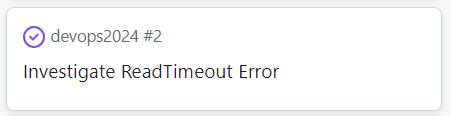
\includegraphics[width=0.6\textwidth]{images/issues.png}
    \caption{\href{https://github.com/DevOps2024-Organization/devops2024/issues/2}{Issues} for fixing Read Time out error}
    \label{fig:github-issues}
\end{figure}

When scaling the application with Docker Swarm, we faced an issue where the Grafana dashboards and login credentials were removed due to creating a new container, which we fixed by adding a volume to the Grafana container, see Figure \ref{fig:grafana-issue}.
Furthermore, Elasticsearch was very performance-heavy, so we upgraded the webserver host with more memory and CPU power.

\begin{figure}[H]
    \centering
    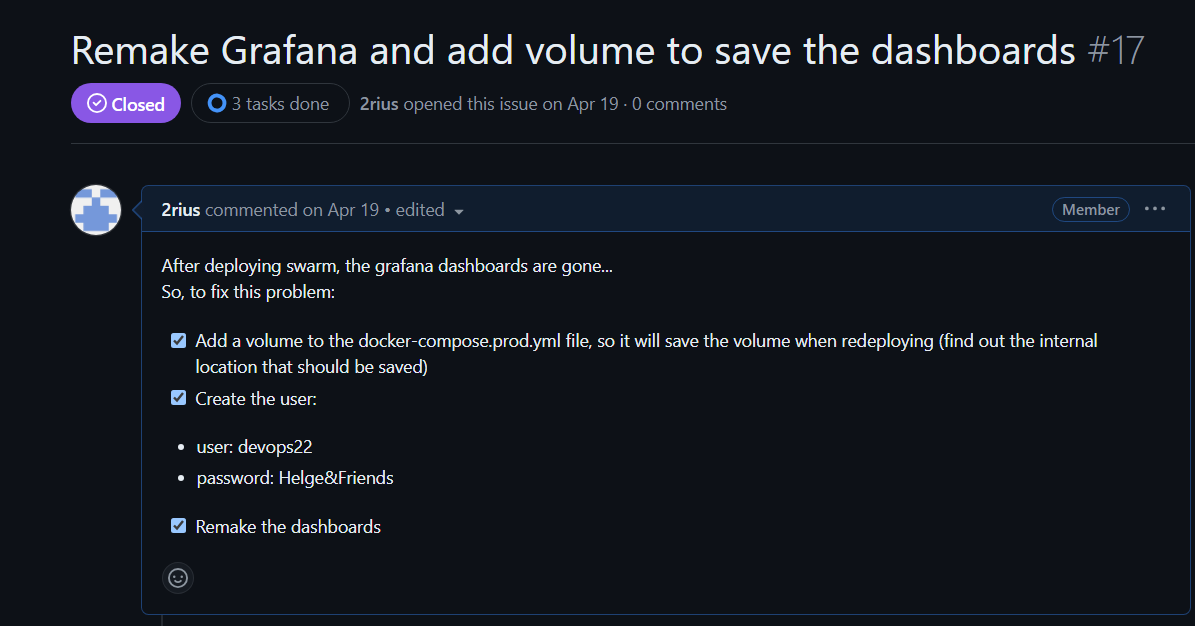
\includegraphics[width=0.8\textwidth]{images/grafana-issue.png}
    \caption{\href{https://github.com/DevOps2024-Organization/devops2024/issues/17}{Issue} about Grafana dashboards disappearing}
    \label{fig:grafana-issue}
\end{figure}

{\raggedright
\bibliographystyle{unsrturl}
\bibliography{bibliography}
}

\appendix

\chapter{Appendix}\label{app}
\section{Artifacts constitutional to the project}

\begin{itemize}
    \item The GitHub repository for the codebase can be found at \href{https://github.com/DevOps2024-Organization/devops2024}{https://github.com/DevOps2024-Organization/devops2024}
    \item The issue tracking can be found at
    \href{https://github.com/orgs/DevOps2024-Organization/projects/1}{https://github.com/orgs/DevOps2024-Organization/projects/1}.
    \item The application can be found at
    \href{http://104.248.43.157:8080/}{http://104.248.43.157:8080/}
    \item The API can be found at
    \href{http://104.248.43.157:5000/}{http://104.248.43.157:5000/}
    \item The Kibana dashboard can be found at
    \href{http://104.248.43.157:5601/}{http://104.248.43.157:5601/}
    \item Grafana Dashboards can be found at \href{http://104.248.43.157:3000/}{http://104.248.43.157:3000/}.
\end{itemize}

\end{document}
